Afin de savoir si les capteurs choisis vont fonctionner, il a fallu effectuer une série de simulations. 
Le premier défi était de simuler de la neige en pleine été. Etant donné que des canons à neige ou autres 
dispositifs du style n’étaient pas disponibles, de la fausse neige a dû être fabriquée. Cependant, simuler 
des chutes de neige implique des importantes salissures. Un banc de test a donc été mis en place pour effectuer 
ces tests de manière propre. Pour simuler la neige qui tombe, un canon a confettis permit de le faire. 
Ces mesures ont grandement aidé à l’avancement du projet.\par 
Le deuxième grand défi était de compacter toute la partie électronique dans un boitier pouvant résister aux 
intempéries. Une carte de développement, un Shield, des batteries ainsi que d’autres composants doivent être 
à l’abri dans ce boitier. Pour assurer des mesures fiables et la survie de l’électronique, l’étanchéité du 
boitier est nécessaire. La simplicité du démontage est aussi recherchée, elle permettra aux personnes de 
gagner du temps lors du montage ou de la maintenance.

\section{Banc de test}

Durant l’étape de réflexions deux capteurs ont été retenus. Cependant les moyens pour essayer ces derniers 
étaient restreints. Afin d’avoir un espace pour effectuer des tests volatiles sans impacter nos collègues, 
un banc d’essai a été mis en place. \\
Le but était d’avoir assez de place dans une zone fermée pour être 3 personnes à l’intérieur tout en créant 
des nuages de confettis. Ces nuages ne devaient en aucun cas gêner les autres personnes dans la salle de classe. 
Une cage avec une base de 2m par 1.5m et 1.5m de haut a été développé. 

\begin{figure}[H]
    \centering
    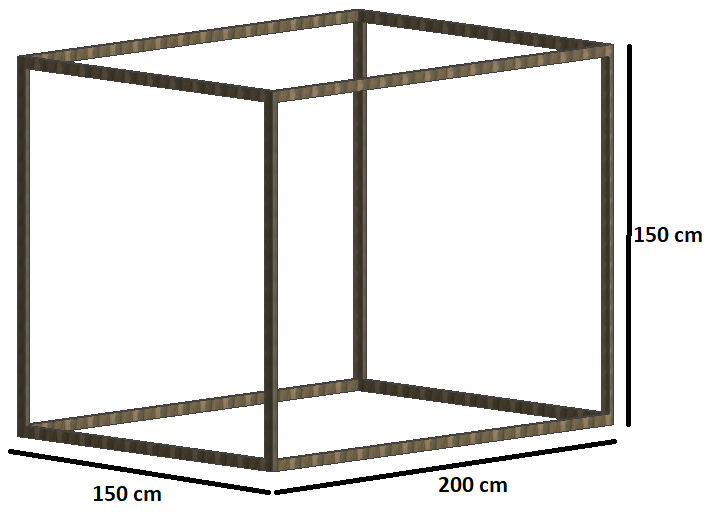
\includegraphics[width=0.3\textwidth]{Images/photos_PGA/P004_CageDeTest21.png}
    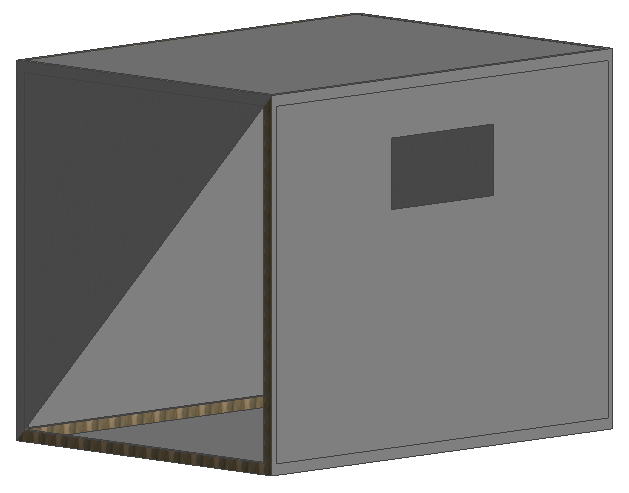
\includegraphics[width=0.3\textwidth]{Images/photos_PGA/P004_CageDeTest2.png}
    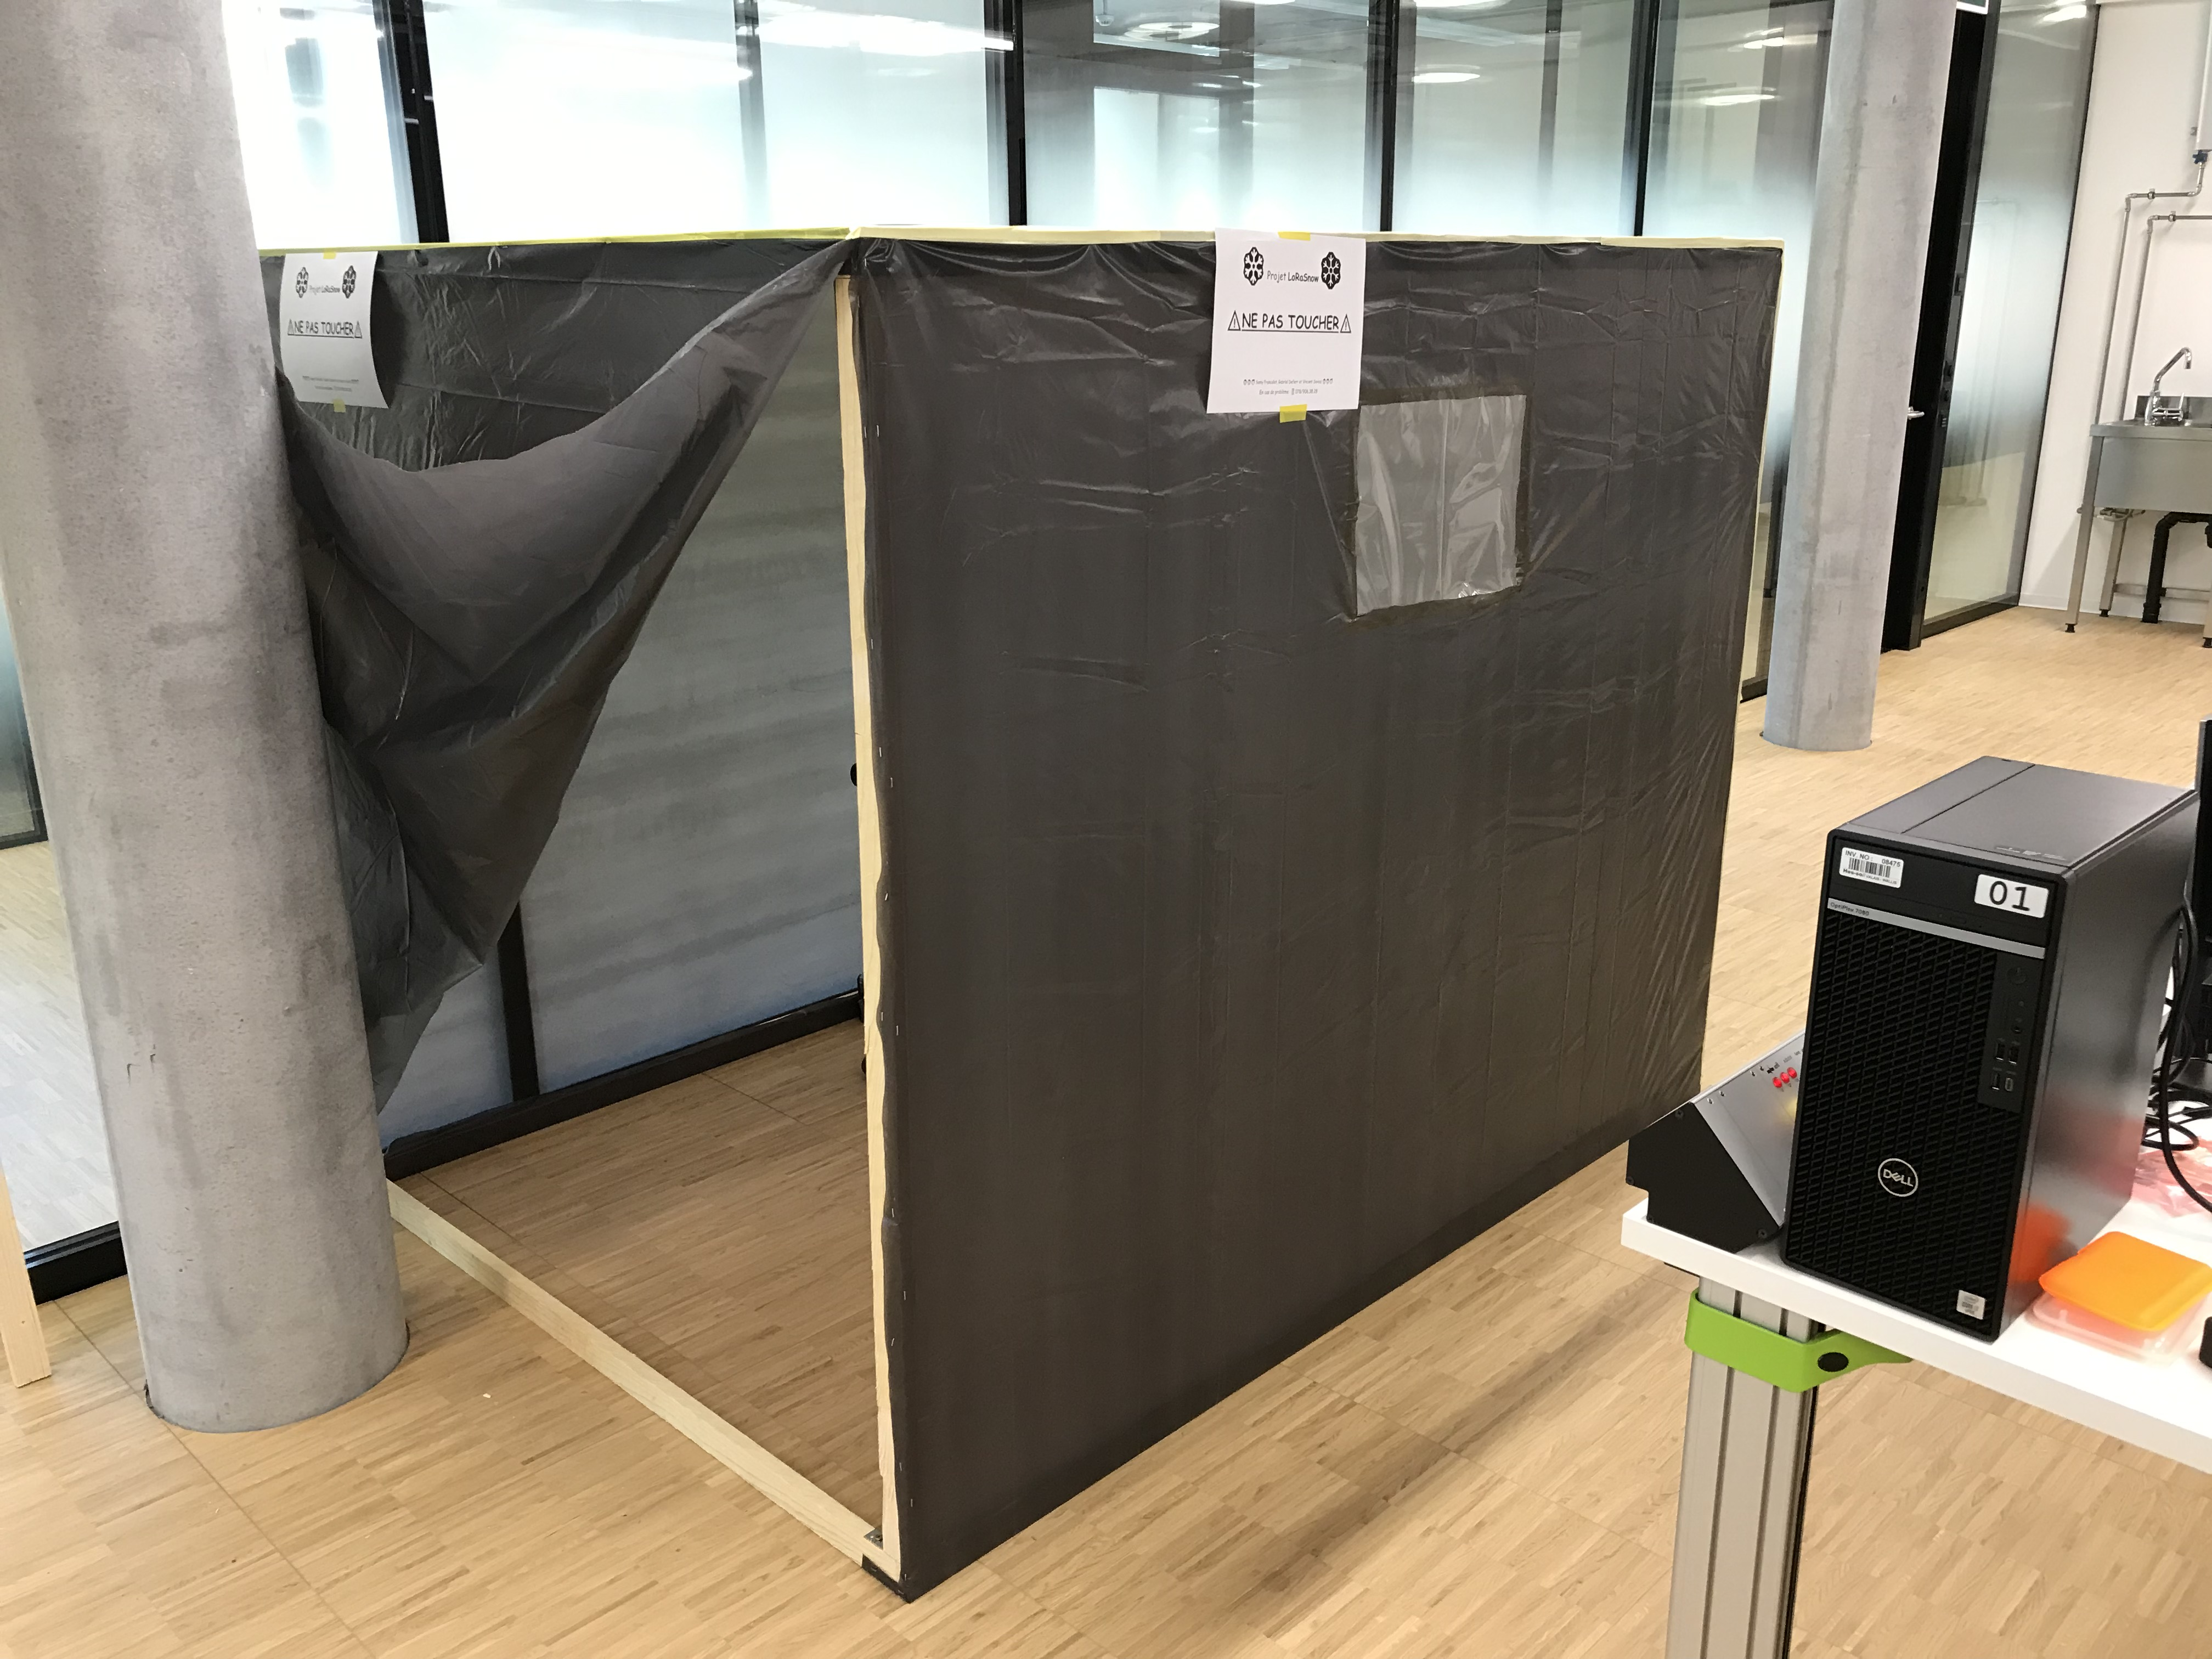
\includegraphics[width=0.3\textwidth]{Images/photos_PGA/IMG_0442.jpg}
    \caption{Encombrement de la structure de test}
    \label{fig:encombrement}
\end{figure}

La structure nécessitait d’être rapidement construite. Sans elle, les essais auraient été bien plus 
compliqués. Une structure en bois a donc été retenue pour sa simplicité à être travaillée. Les façades 
de la cage ont été réalisées avec des bâches de protections épaisses qui furent agrafées sur la structure 
en bois. Les planches en bois ont été assemblées à l’aide d’équerres en métal et de vis à bois. Toutes 
les fournitures ont été trouvées chez Hornbach.\\
Afin d’avoir une très bonne rigidité, la structure aurait pu être triangulé avec des poutres en bois en 
plus. Cependant la structure étant exposé à quasiment aucune contrainte, la rigidité rajoutée par les 
bâches de protections épaisses agrafée était largement suffisante. Cette configuration nous a permis 
d’économiser du temps et de l’argent.

\subsection{Fausse neige (confettis)}

\subsubsection{Problématique}

Simuler de la neige en plein été est quelque chose de compliqué. La température ne jouant pas en notre 
faveur, la solution retenue était d’utiliser des confettis blancs. À la suite d’une commande impossible 
de confettis (rupture de stock), une autre solution dure être trouvée rapidement.

\subsubsection{Méthode}

La première chose envisagée était de regarder dans les bacs des perforatrices automatiques situées 
dans les imprimantes de l’école. Malheureusement ces derniers étaient vidés régulièrement. La quantité 
trouvée était plus qu’insuffisante.\\
La deuxième solution, celle qui a été retenue, était d’utiliser la déchiqueteuse du secrétariat. Cette 
démarche n’était pas des plus écologique, mais elle a permis de pouvoir avoir les confettis rapidement. 
Un paquet de feuille blanche a été détruit pour fabriquer un carton plein de lamelle blanche s’apparentant 
à des confettis ou de la grosse neige. \\
Le remplissage du carton ci-dessous a pris environ une heure. 

\begin{figure}[H]
    \centering
    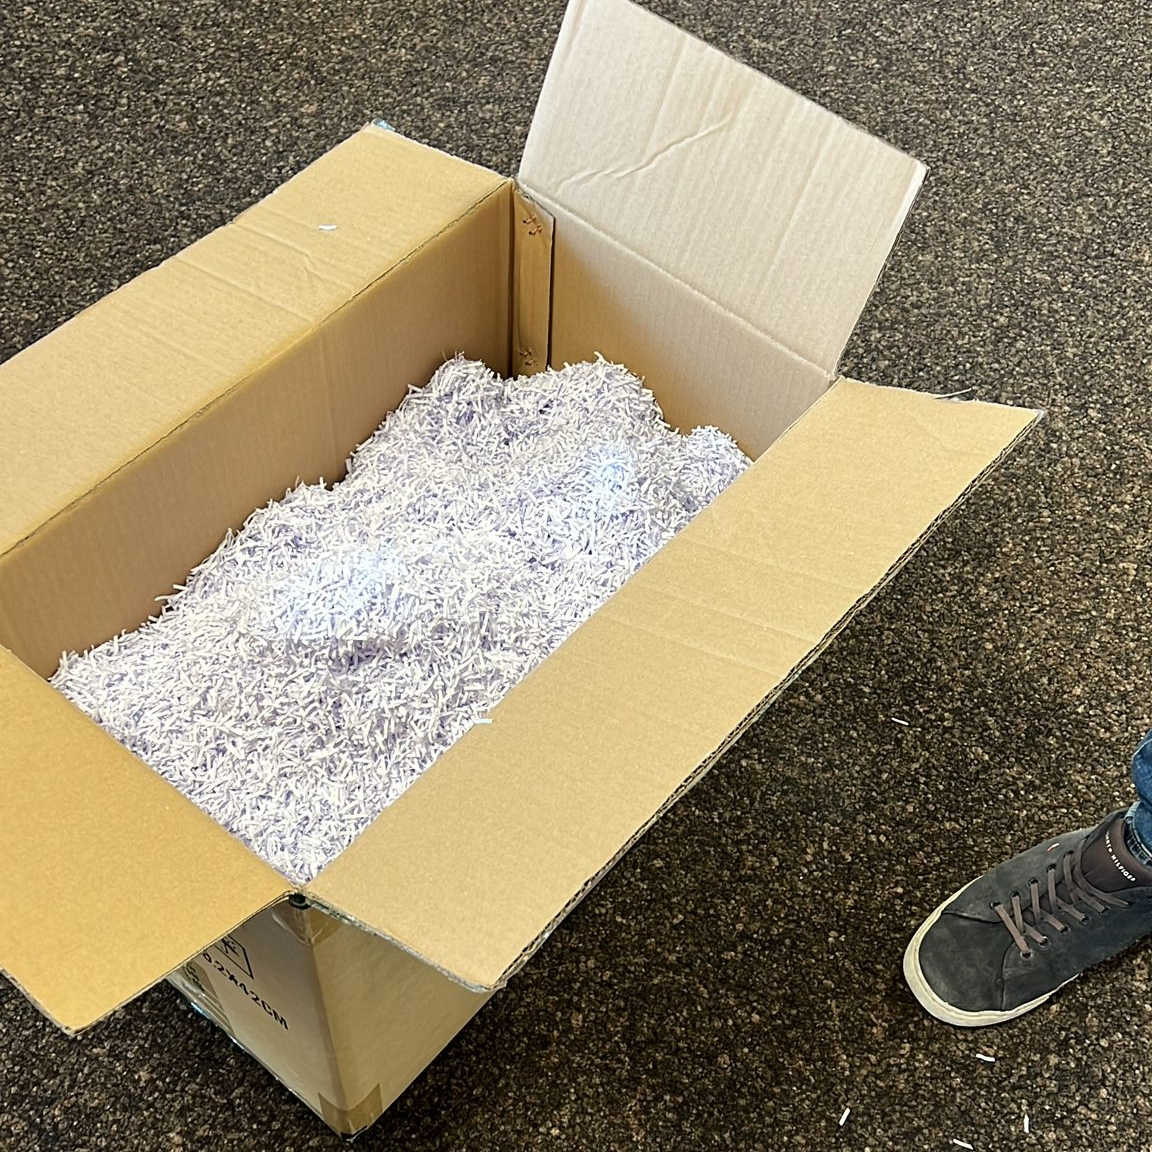
\includegraphics[width=0.4\textwidth]{Images/photos_PGA/ConfBox.jpeg}
    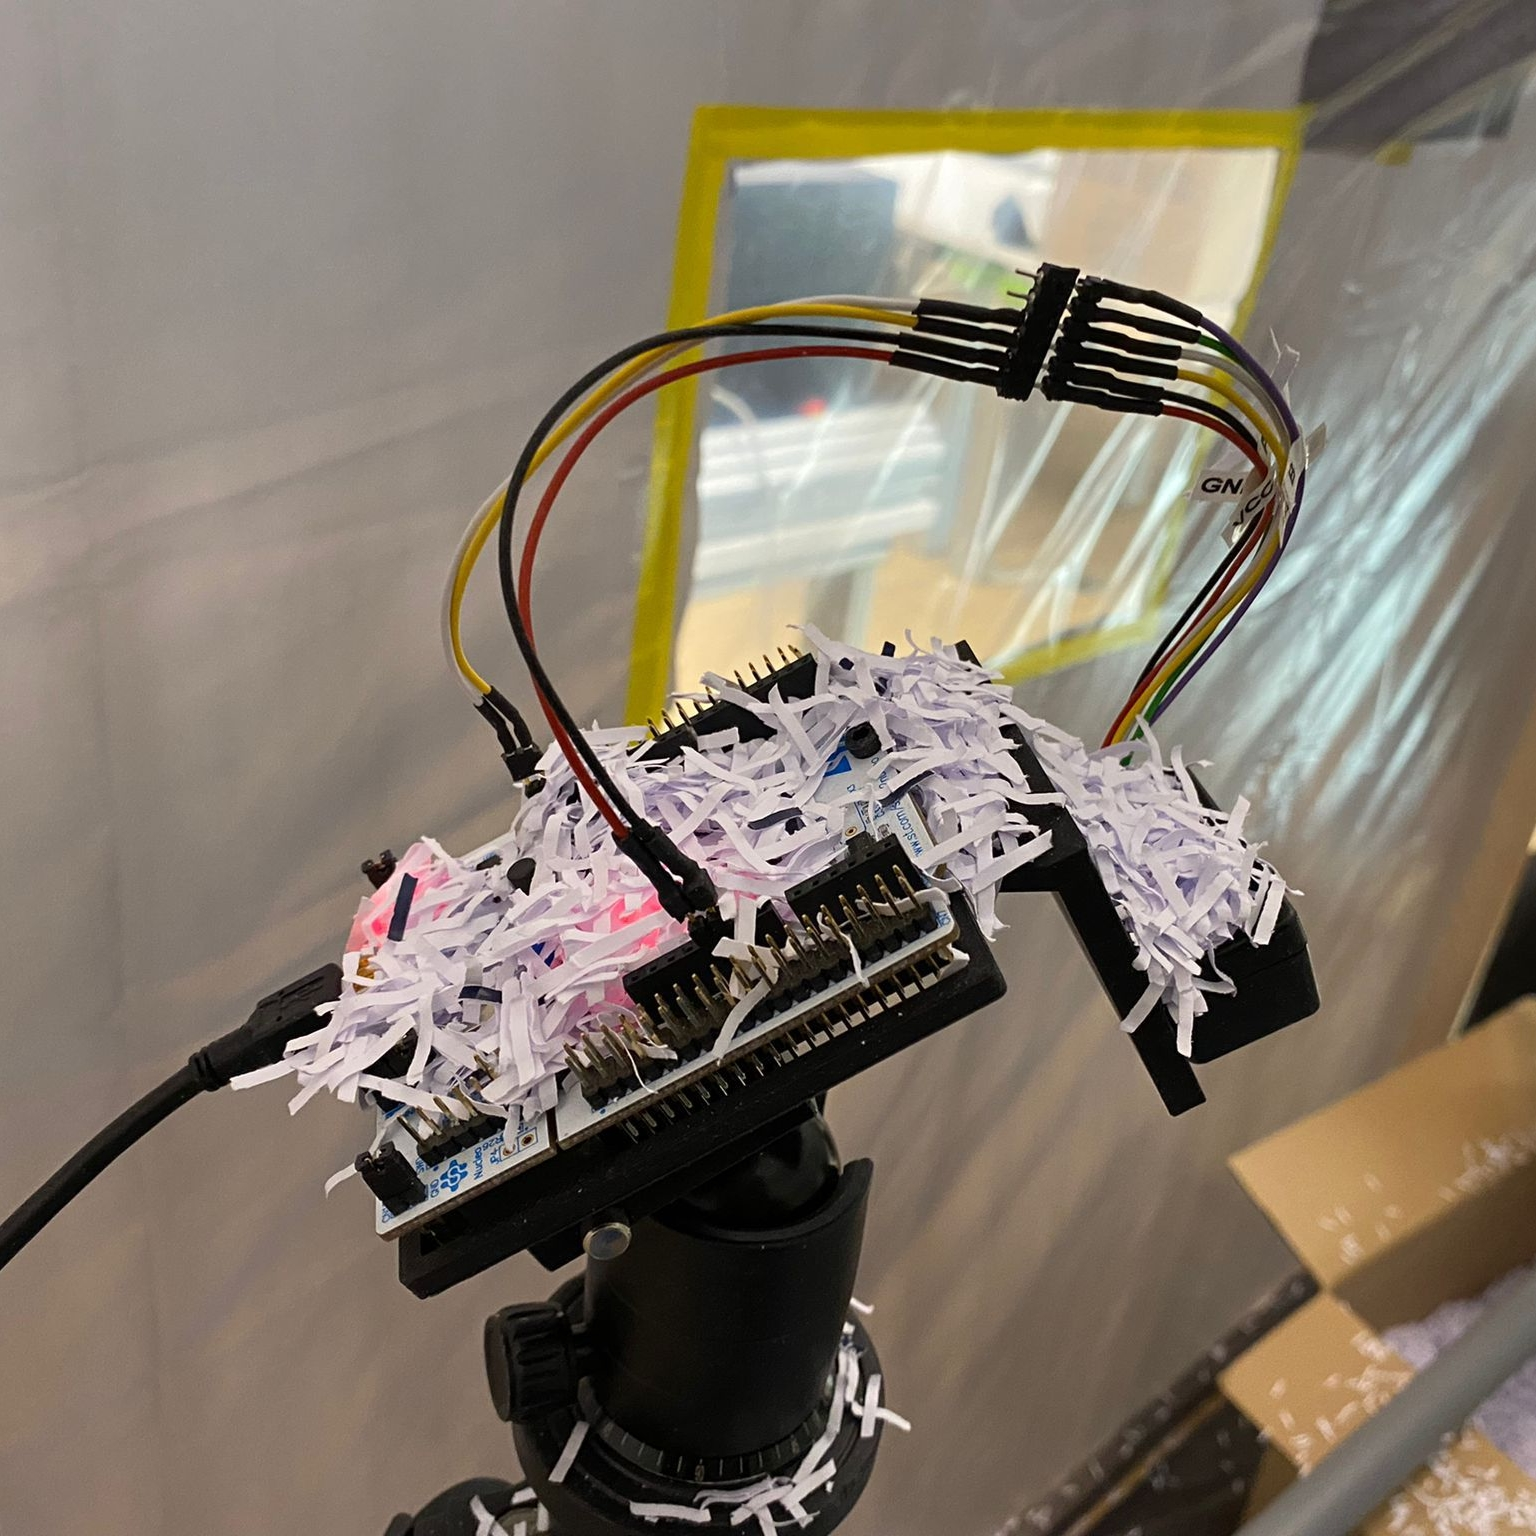
\includegraphics[width=0.4\textwidth]{Images/photos_PGA/conf.jpeg}
    \caption{Aspect des confettis fabriqués}
    \label{fig:confettis}
\end{figure}

\subsection{Canon à confettis}

La meilleure solution pour simuler la chute des flocons est de projeter des confettis de la manière la 
plus continue possible vers le haut. Les premiers essais ont été effectué en les jetant manuellement 
devant les capteurs. Cependant, il fallait avoir un débit constant afin de pouvoir faire des séries de
mesures et déterminer plus précisément les erreurs. 

\subsubsection{Principe de fonctionnement}

En regardant les canons à confettis existants qui la plupart fonctionnent par à-coup d’air comprimé 
(effet non désiré) une solution avec un débit d’air plus faible fonctionnant par effet venturi fut 
retenue. Le principe de base (inspiré des carburateurs) était, grâce à un débit d’air régulier dans 
notre cas, d’aspirer des confettis introduit dans un réservoir grâce à une baisse de pression à un 
endroit précis. La première version se composait d’un tube principal avec une réduction de section. 
Ce tube était parcouru par le débit d’air constant. Un réservoir de confettis se situait au-dessus 
de la zone de dépression (réduction de section). Un petit coude déposé dans le réservoir permettait 
aux confettis de pouvoir mieux couler dans le tube principal.\par 
Sur le schéma ci-dessous, le principe y est bien représenté. Le débit d’air constant en noir arrive 
au niveau du réservoir, la section diminuant la pression diminue aussi. En diminuant une dépression 
a ce niveau est créé, un phénomène d’aspiration ce produit. En ressortent de ce système, un mélange 
d’air et de confettis.

\begin{figure}[H]
    \centering
    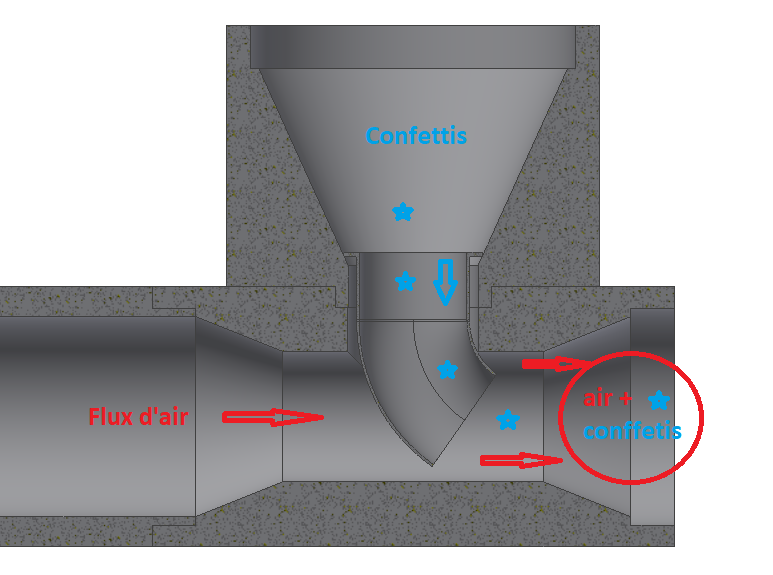
\includegraphics[width=0.5\textwidth]{Images/photos_PGA/venturi_v1b.PNG}
    \caption{Principe du canon à effet Venturi}
    \label{fig:venturi}
\end{figure}

Cette première version fut rapidement envoyée dans l’atelier pour être imprimée en 3d afin d’effectuer 
les premiers tests et les éventuelles corrections du canon. Voici une photo du tube principale imprimé 
en PETG grâce à l’imprimante 3d de l’école.

\begin{figure}[H]
    \centering
    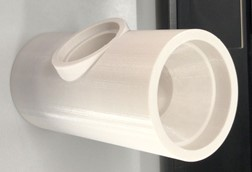
\includegraphics[width=0.5\textwidth]{Images/photos_PGA/CanonBloc.jpg}
    \caption{Exemple d'impression 3D du canon}
    \label{fig:3DPrintCanon}
\end{figure}

\subsubsection{Turbine}

Un paramètre indispensable était d’avoir une source d’air continue avec un bon débit. La classe étant 
équipée d’air comprimé, il suffisait de l’utiliser pour avoir un bon débit d’air constant. Cependant, 
le bâtiment étant encore pas terminé les raccords d’air n’était pas fixé. Une autre solution demandait 
à être trouvée. Il se trouve, qu’une turbine alimentée par un moteur à courant continue était la bonne 
solution. Premièrement, ce dispositif est assez simple, pour régler la vitesse de rotations il suffit 
de changer le voltage aux bornes du moteur. Deuxièmement la mécanique est très facilement intégrable 
au canon. Cette solution permit de ne plus se soucier des histoires de débit d’air.

\begin{figure}[H]
    \centering
    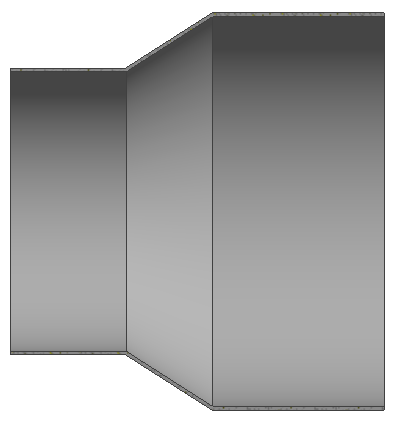
\includegraphics[width=0.35\textwidth]{Images/photos_PGA/adaptmotventi.PNG}
    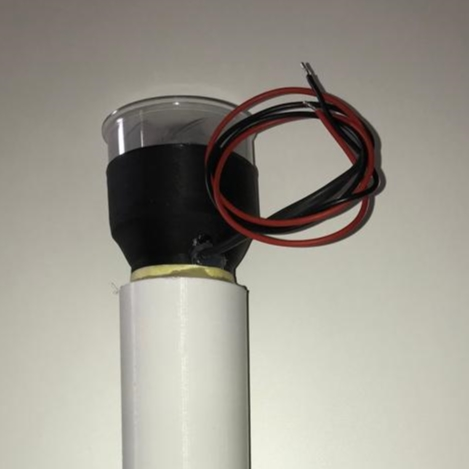
\includegraphics[width=0.4\textwidth]{Images/photos_PGA/zoomTurbine.jpg}
    \caption{Turbine DC}
    \label{fig:turbine}
\end{figure}

\subsubsection{Problèmes rencontrés}

A la suite de plusieurs tests, plusieurs choses se sont révélées problématiques. Premièrement, les 
confettis « maison » ont une fâcheuse tendance à s’enchevêtrer les uns dans les autres, cela réduit 
considérablement leurs capacités à bien couler dans le réservoir. Ce dernier se retrouvait sans cesse 
bouché. Grace aux tests, le fait d’agrandir le passage des confettis permettrai d’avoir un meilleur 
écoulement et de limiter la formation des bouchons.

\subsubsection{Solution apportée}

En prenant compte des problèmes survenu lors des premiers essais, une deuxième version fut modélisée. 
Cette fois ci avec un réservoir plus grand et un angle de remplissable plus faible. Le coude passe 
de 28mm de diamètre à 34 mm et cette fois ci il est imprimé directement sur le tube principal afin 
d’éviter les angles trop saillants qui pourraient causer un blocage. Afin d’obtenir un coude plus large 
il a fallu augmenter le changement de section dans le tube principale. Refaire complètement la pièce 
pour tout faire plus grand aurait possible pour avoir plus d’aspiration. Cependant, le fait de garder 
les dimensions de bases permettait de gagner du temps et d’éviter d’avoir à refaire des impressions 
pour rien ou de racheter du matériel en plus.

\begin{figure}[H]
    \centering
    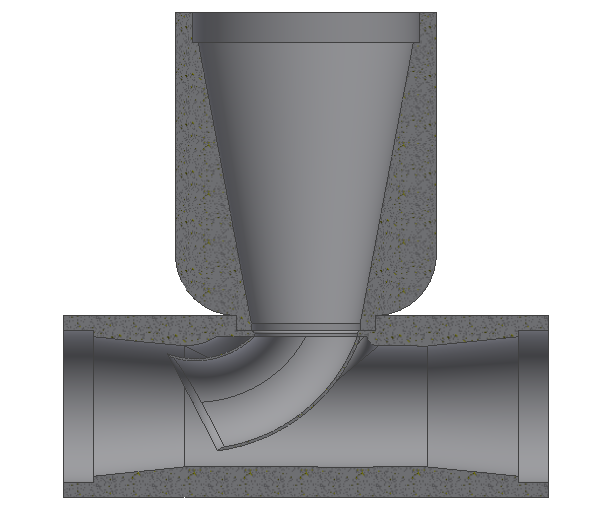
\includegraphics[width=0.4\textwidth]{Images/photos_PGA/venturi_v2.PNG}
    \caption{Deuxième version du canon}
    \label{fig:venturiv2}
\end{figure}

Lors des essais de la nouvelle version, le changement était notable. Le fait d’avoir augmenté le diamètre 
du coude et de l’avoir imprimé en une fois avec le tube principal a réduit fortement les angles saillants. 
Les lamelles de papiers continuaient à se coincer de temps en temps mais l’objectif d’avoir un débit 
constant pendant une bonne minute a pu largement être atteint. Le canon était même capable s’il était 
placé réservoir vers le bas d’aspirer les confettis comme un aspirateur et de les rejeter comme de la 
neige. 

\begin{figure}[H]
    \centering
    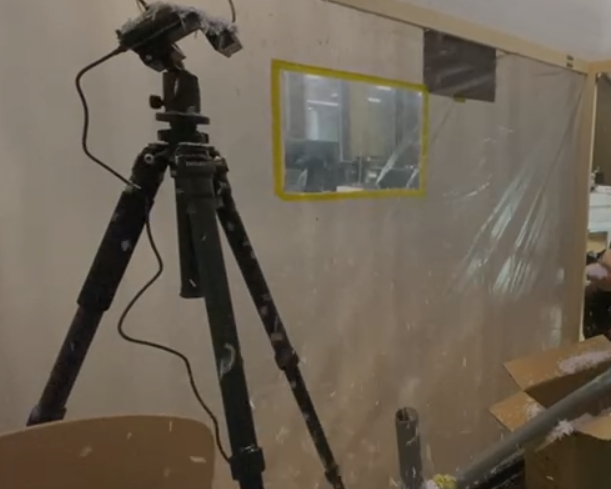
\includegraphics[width=0.4\textwidth]{Images/photos_PGA/canonAction1.PNG}
    \includegraphics[width=0.4\textwidth]{Images/photos_PGA/canonAction2.PNG}
    \caption{Mise en fonction du canon}
    \label{fig:canonupdate}
\end{figure}

Pour l’assemblage des différentes pièces du canon, comme ces dernières étaient très bien ajustées et 
tenaient sans rien entres elles, le fait d’utiliser des colles fortes spécifiques n’a pas été nécessaire. 
L’utilisation de colle chaude pour garantir un non-détachement et un démontage plus simple fut utilisé. 
Certaines pièces étant interchangeable, elles ne pouvaient pas être collé, l’utilisation de scotch pour 
garantir aucun déboitement fut très pratique. Cet appareil a surtout été conçu dans un but d’avancer 
les mesures rapidement et le temps de conception/réalisation était très court, c’est pourquoi la complexité 
des fixations n’a pas été la priorité. L’objectif qui était d’avoir un débit de neige constant a donc 
été atteint.

\begin{figure}[H]
    \centering
    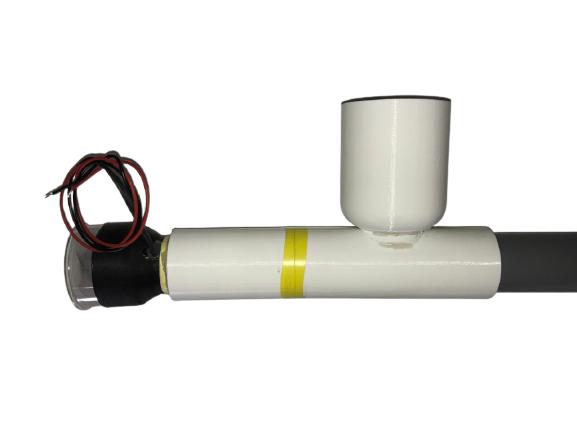
\includegraphics[width=0.4\textwidth]{Images/photos_PGA/canonComplpetv2-removebg-preview.png}
    \caption{Ensemble final du canon à confettis}
    \label{fig:canonensemble}
\end{figure}

\section{Boitier}

\subsection{Premier prototype}

\subsubsection{Ouverture}

À la suite de ça un prototype de boitier fut réalisé pour se rendre compte de l’encombrement, de la 
praticité et du design. Le choix de l’ouverture était de la mettre à l’arrière du boitier avec le 
système d’étanchéité démontré ci-dessus. Le maintien de la pression sur le joint était fait grâce à 
4 vis qui venait directement prendre dans la base du boitier. Cette manière de fixer permet de ne 
pas avoir de trou traversant le boitier. Cette méthode est la même que sur celle de la plupart des 
boitier étanche.

\begin{figure}[H]
    \centering
    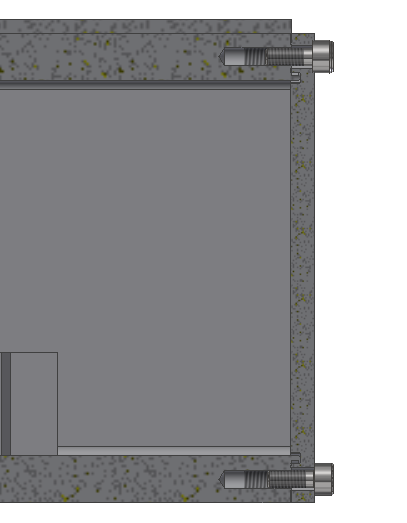
\includegraphics[width=0.4\textwidth]{Images/photos_PGA/Arrièreboitierv3coté.PNG}
    \caption{Ouverture arrière du boitier}
    \label{fig:vuearriereboitier}
\end{figure}

\subsubsection{Encombrement}

En ce qui concerne l’encombrement de la carte de développement dans le boitier qui faisait 200mm de 
long par 100mmx100mm, il y avait juste assez de place. Dans le cas ci-dessous il manque les batteries, 
le capteur et le Shield.

\begin{figure}[H]
    \centering
    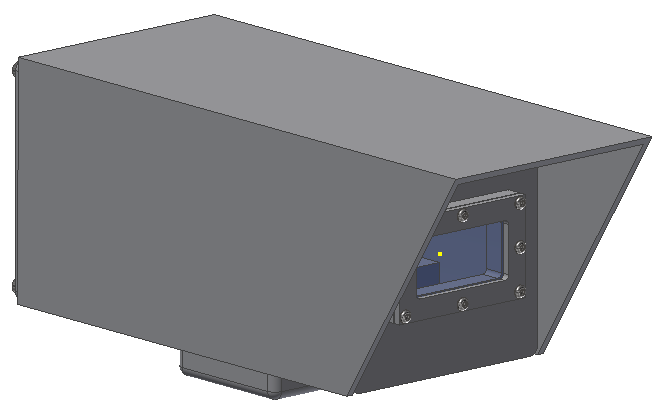
\includegraphics[width=0.3\textwidth]{Images/photos_PGA/boitierV3.PNG}
    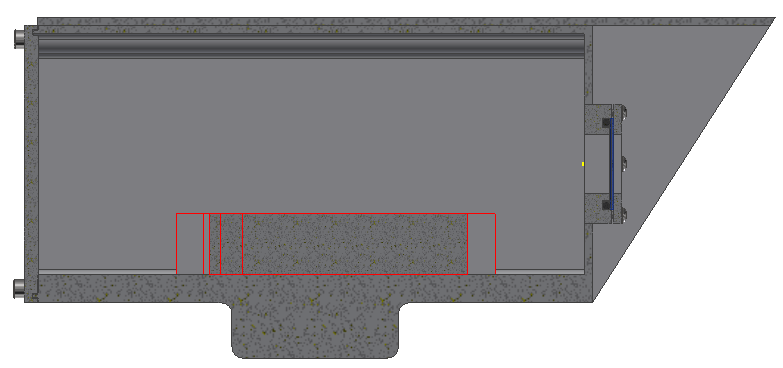
\includegraphics[width=0.4\textwidth]{Images/photos_PGA/boitierV3enc.PNG}
    \caption{Encombrement du boitier, version 1}
    \label{fig:encombrementv1}
\end{figure}

En avançant dans le design du boitier des difficulté quant à la fixation de l’électronique dans le boiter 
se manifestèrent. L’utilisation d’une casquette devenait aussi complexe, ce n’est pas facile de devoir 
fixer des choses sur un boitier sans faire des trous traversants. La fixation pour le bras était pensée 
sous le boitier, cependant elle aurait aussi pu être prise sur les côtés en englobant la casquette. 
À la suite de tous ces problèmes, le design fut complètement revisité.

\subsection{Version finale du boitier}

Le dernier design est inspiré des caméras de surveillance récente. Ce boitier sera conçu à base de 
polymère. Cette matière permet de limiter les transferts de chaleurs et les couts.

\subsubsection{Matériaux}

Matière
Les deux matériaux les plus souvent retrouvés dans l’industrie pour les boitiers sont l’Acrylonitrile 
butadiène styrène (abs) et le polycarbonate (pc). Le polycarbonate n’apprécie pas d’être exposé trop 
longtemps à un environnement humide. Cela pourrait provoquer de l’hydrolyse et dégrader le boitier. 
L’abs quant à lui est très résistant, il est notamment utilisé pour faire des barques de secours.  
L’injection de l’abs est très rependue, ce matériau est notamment utilisé pour fabriquer les briques Lego. 
Ce terpolymère montre une bonne résistance aux chocs jusqu'à -40 °C . Sa TG se situe aux alentours 110 
degrés, ce qui est largement suffisent dans notre cas. Le problème de l’abs est qu’il a une mauvaise 
résistance aux UV. L’utilisation d’un revêtement de protection UV sous forme de peinture est envisageable. 
Ce processus permettrait d’augmenter la durée de vie du boitier. Le prix de l’abs se situe aux alentours 
de 3200 euros la tonne\footnote{https://www.polyvia.fr/fr/prix-du-plastique-les-previsions-pour-2022}.\\
L’aluminium aurai aussi pu être intéressant pour la fabrication de ce boitier. Cependant la fonderie 
s’avère plus complexe et plus couteuse que l’injection plastique. Le prix de la matière serait quasiment 
triplé. Les caractéristiques du polymère étant parfaitement suffisant, l’intérêt d’utiliser de l’aluminium 
n’était donc pas nécessaires.

\subsubsection{Ouverture}

L’ouverture se fait par en haut à l’aide d’un couvercle amovible. Le système de d’étanchéité est le 
même que pour les précédentes versions. Le maintien en pression sur le joint est effectué grâce à 
une fixation dites grenouillère. La grenouillère dispense l’utilisation d’outils et permet un gain 
de temps lors de l’ouverture et la fermeture. Cette dernière possède une serrure intégrée pour dissuader 
des possibles vols.

\begin{figure}[H]
    \centering
    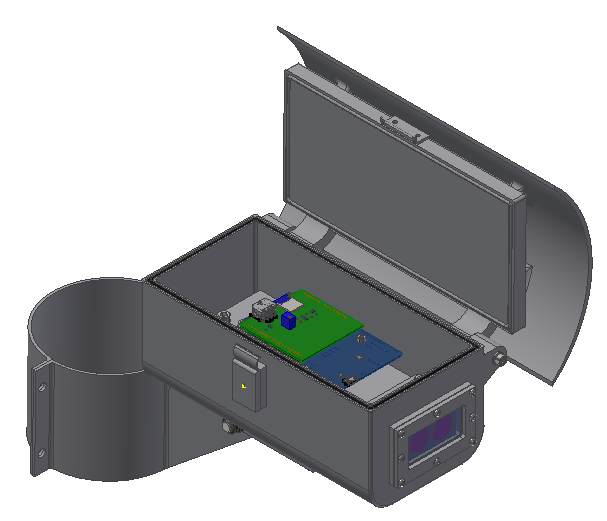
\includegraphics[width=0.4\textwidth]{Images/photos_PGA/Boitierv41.PNG}
    \includegraphics[width=0.35\textwidth]{Images/photos_PGA/grenouillère.PNG}
    \caption{Ouverture du boitier, version 2 (à gauche), grenouillère pour la fermeture (à droite)}
    \label{fig:ouverturev2}
\end{figure}

\subsubsection{Pivot du couvercle}

L’une des grandes forces de ce systèmes est son ouverture simplifiée. En effet, le couvercle est fixé 
comme une trappe. Cette spécificité permet d’avoir un bien meilleur accès à l’intérieur du système. 
Cette particularité permet pouvoir manipuler aisément les éléments qui se situent à l’intérieur. Le 
pivot est assuré par un axe (tube) fileté à ses deux extrémités. Deux vis viennent maintenir de chaque 
côté l’axe afin qu’il ne puisse pas sortir de son logement.

\begin{figure}[H]
    \centering
    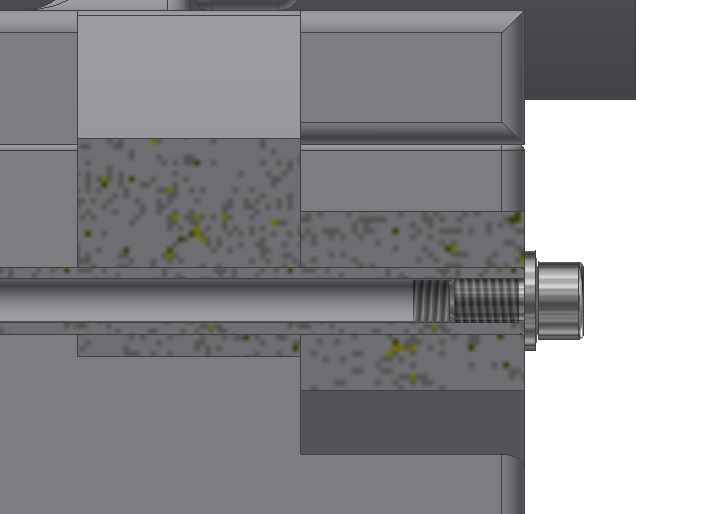
\includegraphics[width=0.25\textwidth]{Images/photos_PGA/pivotcoupe.PNG}
    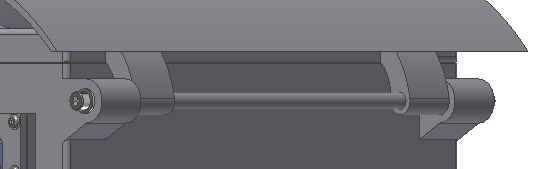
\includegraphics[width=0.6\textwidth]{Images/photos_PGA/pivotnormal.PNG}
    \caption{Mécanisme du pivot}
    \label{fig:pivot}
\end{figure}

\subsubsection{Fixation de la casquette}

La casquette qui se situe sur le couvercle est facilement démontable pour mettre un autre modèle ou 
la changer en cas de dégradation Elle est fixée par 4 vis imbus qui viennent se loger dans des inserts 
situés sur le dessus du couvercle. Les fixations de la casquette sont posées sur le couvercle, cette 
configuration permet de soulager les efforts sur les supports.

\begin{figure}[H]
    \centering
    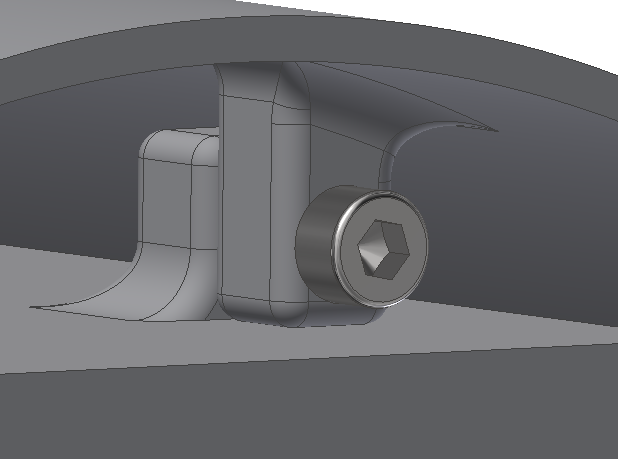
\includegraphics[width=0.4\textwidth]{Images/photos_PGA/fixcasquette.PNG}
    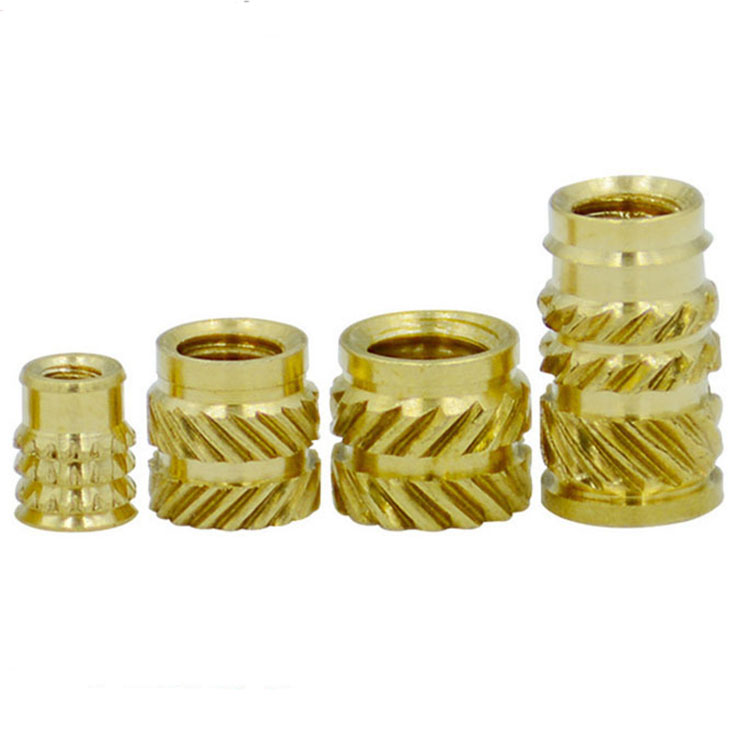
\includegraphics[width=0.4\textwidth]{Images/photos_PGA/inserts.jpg}
    \caption{Mécanisme du pivot}
    \label{fig:casquette}
\end{figure}

\subsubsection{Fixation du module}

En ce qui concerne la partie intérieure, 4 supports sont intégrés dans le fond du boitier. Ces derniers 
sont dimensionnés pour accueillir des inserts plastiques. Toute la partie électronique pourra par la 
suite venir fixer sur le dessus. Mettre une vue en coupe avec la plaque de base fixée

\begin{figure}[H]
    \centering
    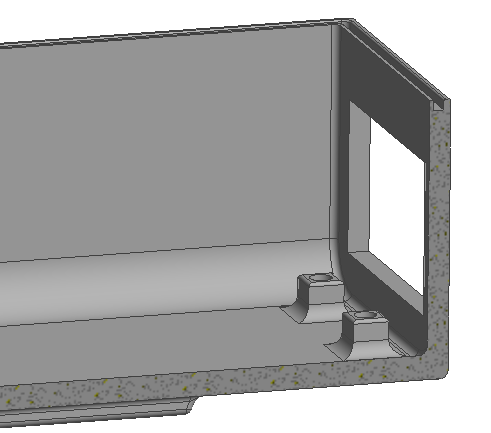
\includegraphics[width=0.4\textwidth]{Images/photos_PGA/fixationbaseModule.PNG}
    \caption{Fixation du module}
    \label{fig:fixbase}
\end{figure}

\subsubsection{Fixations des supports}

La fixation du bras sera assurée par 4 écrou carrés situé sous le boitier. Cette solution permet de 
ne pas à avoir à faire de trous dans le boitier pour maintenir une bonne étanchéité. C’est écrou sont 
guidés dans une gorge afin d’être maintenu pendant le serrage. Le même principe est utilisé dans pour 
fixer des éléments dans les armoires en automation.

\begin{figure}[H]
    \centering
    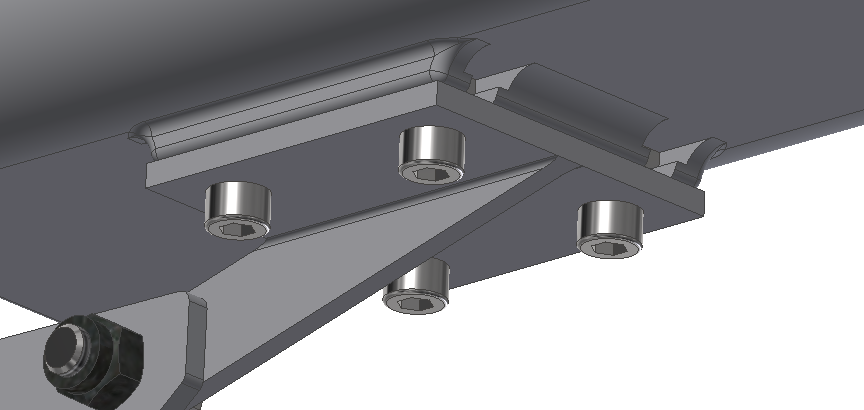
\includegraphics[width=0.4\textwidth]{Images/photos_PGA/fixdessous2.PNG}
    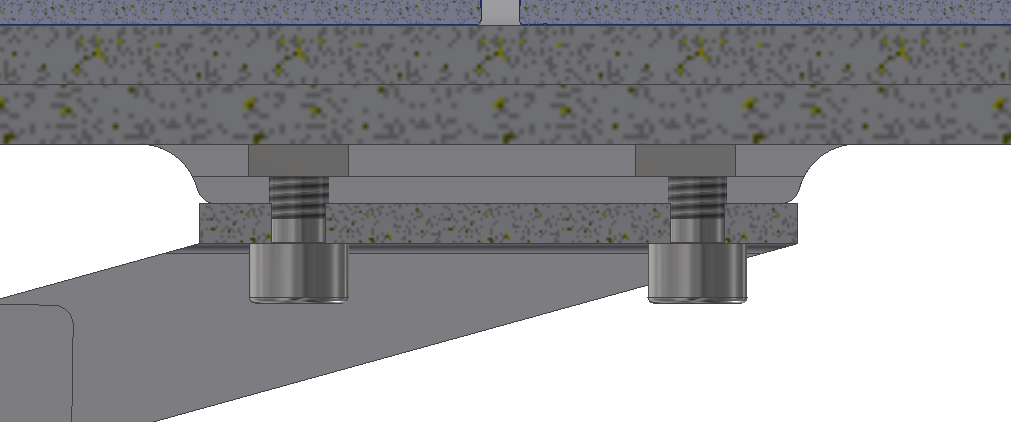
\includegraphics[width=0.4\textwidth]{Images/photos_PGA/écroucarré.PNG}
    \caption{Support de fixation du boitier}
    \label{fig:supportfix}
\end{figure}

\subsection{Module électronique}

Cette partie est consacré au développement d’un module compact et simple composé de toute la partie 
électronique. Ce module est fixé dans le boitier grâce aux 4 plots de fixations situés dans le fond 
du boitier. L’interet de faire une construction mécanique est de pouvoir soutenir tous les composants 
pour les empechers de se déplacer a leur guise. La simplicitée recherchée dans sa conception permetterai 
aux opérateurs de gagner beaucoup de temps.

\begin{figure}[H]
    \centering
    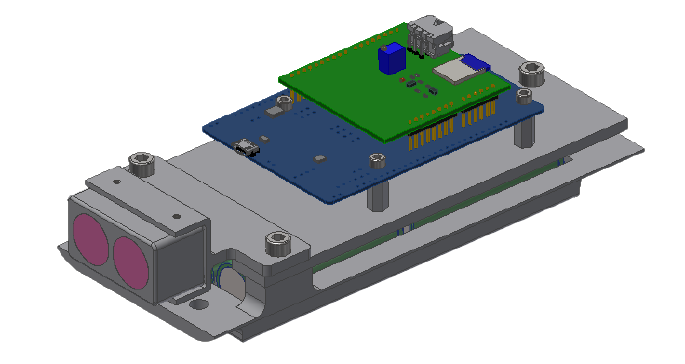
\includegraphics[width=0.6\textwidth]{Images/photos_PGA/ModuleElec2-removebg-preview.png}
    \caption{Module électronique}
    \label{fig:elmodule}
\end{figure}

\subsubsection{Base du support des batteries}

La pièce de base est prévue pour accueillir 6 batteries 18650. Un espace légèrement plus grand est 
prévu. L’appellation 18650 signifie que l’élément rechargeable fait un diamètre de 18mm et une longueur 
de 65mm. Des petites fentes furent aussi pensées pour faciliter un câblage série/parallèle entre les 
éléments. Cette pièce est la fondation du module électronique, elle sera naturellement fixée dans le 
boitier. Cette pièce est directement fixée dans le boitier grâce aux 4 trous de fixations.

\begin{figure}[H]
    \centering
    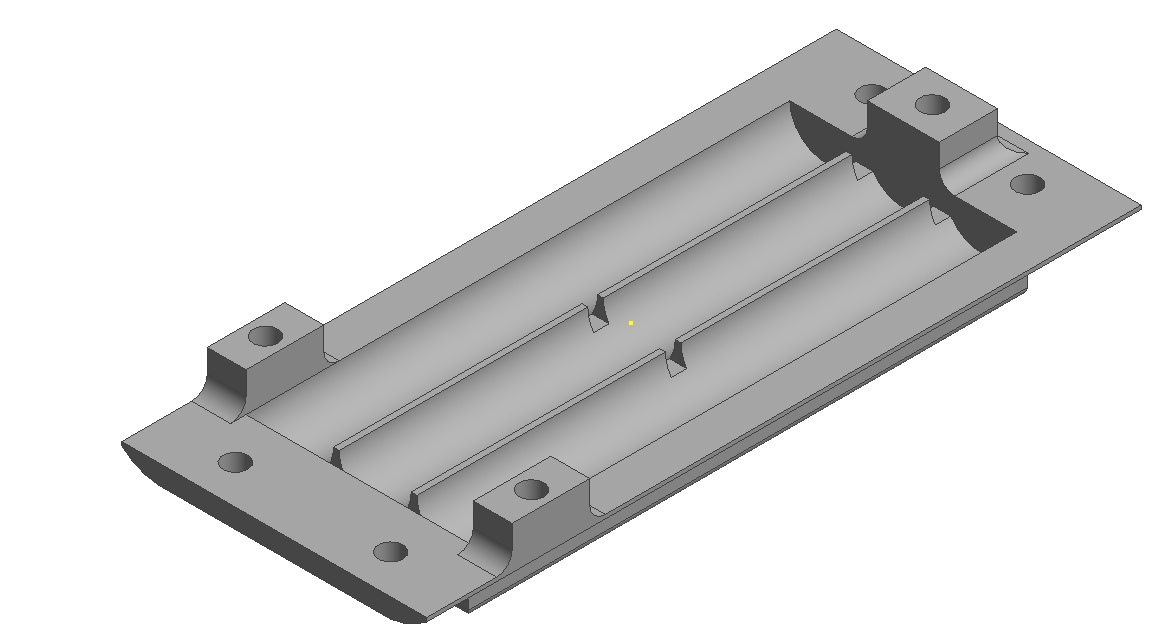
\includegraphics[width=0.4\textwidth]{Images/photos_PGA/moduleFondbat.PNG}
    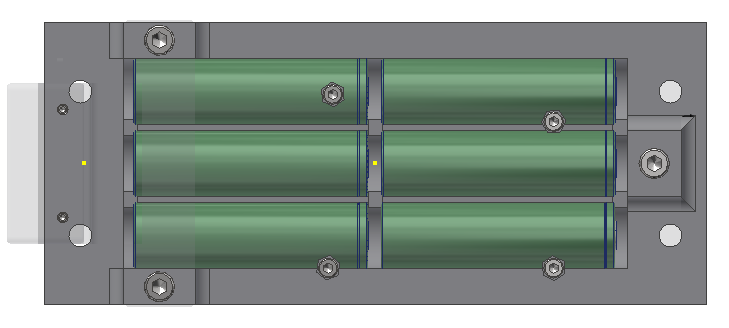
\includegraphics[width=0.4\textwidth]{Images/photos_PGA/bateriebl.PNG}
    \caption{Support à batteries}
    \label{fig:supportbatteries}
\end{figure}

\subsubsection{Plaque de fixation et PCB}

Au-dessus de la pièce supportant les batteries, une plaque est fixée. Cette plaque est très importante 
dans l’ensemble. C’est en quelques sorte la carte mère de l’ensemble. Tous les modules sont fixés autours 
d’elle.  Elle permet grâce aux trois fixations situées aux extrémités de venir bloquer les batteries 
pour pas quelles ne sortent de leurs logements. Ces trois trous sont prévus pour venir fixer la plaque 
sur le module de bas.  Les 4 autres trous servent à fixer la partie PCB. 4 vis à tête fraisée seront 
insérées dans les trous fraisés afin de venir fixer des entretoises en plastiques. Sur ces entretoises 
en plastique les circuits imprimés pourront être fixé à l’aide de visses en plastiques. Ces composants 
plastique permettent d’éviter tout risque de court-circuit.

\begin{figure}[H]
    \centering
    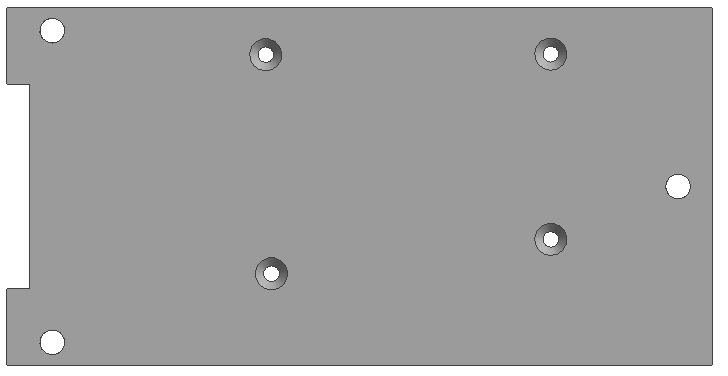
\includegraphics[width=0.4\textwidth]{Images/photos_PGA/plaquesmodule.PNG}
    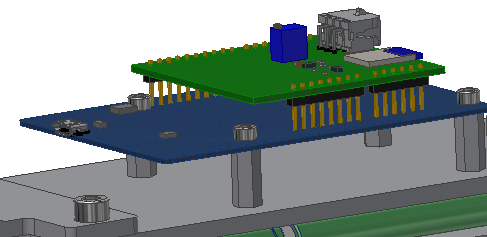
\includegraphics[width=0.4\textwidth]{Images/photos_PGA/PCB.PNG}
    \caption{Plaque de fixation pour la partie électronique}
    \label{fig:fixelectronique}
\end{figure}

\subsubsection{Support du LiDAR}

Le capteur Lidar ne possède pas de trou de fixation, seul deux fentes sont disponibles pour venir 
clipser un support sur ce dernier. Le fabricant préconise de le fixer avec des colsons ou du scotch 
double face. Ces solutions sont plutôt prévues à des fins de bricolage. Des essais de supports à base 
de clips ont été réalisé mais l’ajustement de ces derniers était problématique. C’est pour ça que la 
solution de pincer le capteur à l’aide de vis sans tête est parvenue comme la plus sûre et la plus simple. 
Le support qui permet de fixer le lidar dans la bonne position vient directement se fixer dans les 
trous de fixations du support à batteries.

\begin{figure}[H]
    \centering
    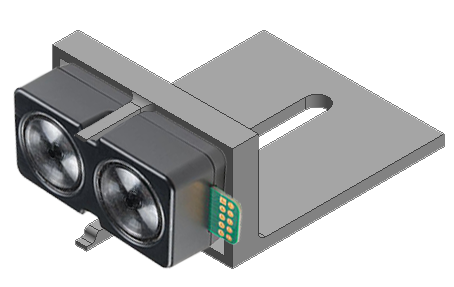
\includegraphics[width=0.3\textwidth]{Images/photos_PGA/lidar dans support.png}
    \includegraphics[width=0.3\textwidth]{Images/photos_PGA/supportLidar2.PNG}
    \includegraphics[width=0.3\textwidth]{Images/photos_PGA/supportlidar.PNG}
    \caption{Support pour le LiDAR}
    \label{fig:supportlidar}
\end{figure}

\subsection{Bras de fixation}

La partie fixation permet d’assurer un positionnement juste et précis de l’ensemble du boitier. Cette 
fixation doit pouvoir se faire sur quasiment toutes les surfaces à dispositions comme les murs ou les 
lampadaires.

\subsubsection{Support du boitier}

Le support du boitier est une partie rigide en aluminium qui vient se visser sous le boitier à l’aide 
e 4 vis. Cette pièce est en deux partie. La première partie est une plaque carrée ayant les trous de 
perçage correspondant au boitier. La deuxième est une autre plaque percée soudée perpendiculairement. 
Ce perçage permettra de jongler entre les systèmes de fixation désiré. Grace à cette liaison par boulon, 
l’inclinaison du boitier pourra être réglée.
En ce qui concerne le réglage précis de l’angle, un petit cadran autocollant pourrait être rajouté 
sur le support et une ligne autocollante sur le support du boitier. Elle permettra de lire la valeur 
de l’inclinaison du boitier. Cette petite subtilité permettra de faciliter le montage du boitier et 
de pouvoir contrôler si la position du boitier est bonne sur le long terme.

\begin{figure}[H]
    \centering
    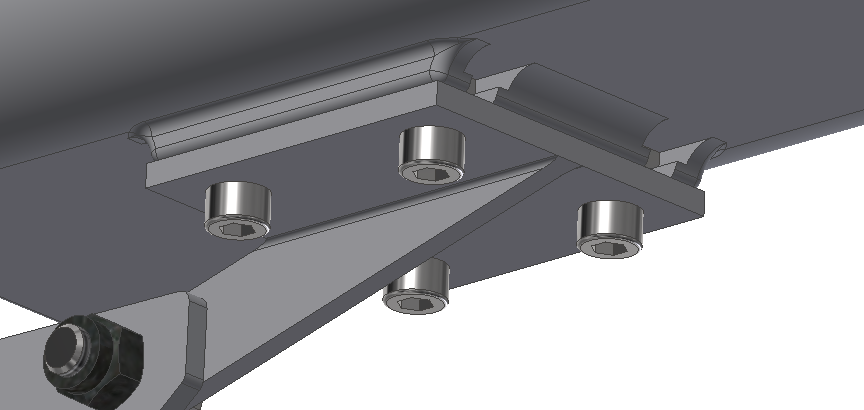
\includegraphics[width=0.4\textwidth]{Images/photos_PGA/fixdessous2.PNG}
    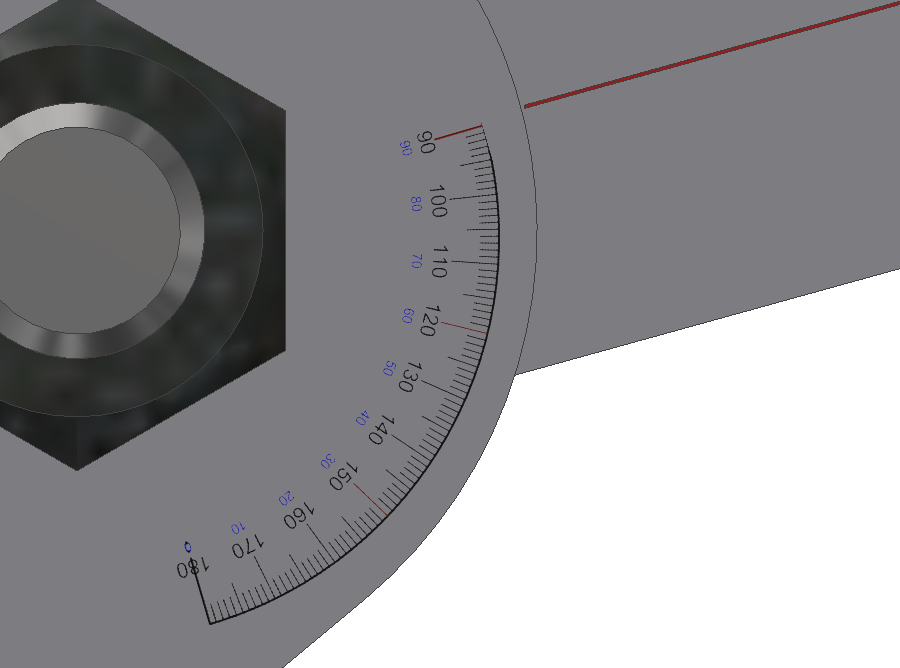
\includegraphics[width=0.4\textwidth]{Images/photos_PGA/mesure d'angle.PNG}
    \caption{Système de réglage de l'élévation}
    \label{fig:angle}
\end{figure}

\subsubsection{Support mural et tubulaire}

L’objectif voulu était de pouvoir fixer le boitier sur des lampadaires ou des poteaux. Un système de 
collier de serrage a donc été conçu pour répondre à cette problématique. Les deux arcs de cercle collé 
entre eux forment un ovale avec une air un peu plus petite que celle du poteau de fixation. En venant 
serrer les vis, une force de serrage agira naturellement sur le poteau et le boitier sera bien fixé. 
Afin de régler la rotation azimutale, c’est-à-dire autours de l’axe du lampadaire, il suffit de placer 
le boitier dans la position voulue. Une fois cette position atteinte, il faut bloquer l’ensemble boulonné. 
Ce dispositif permet deux degrés de liberté, l’azimut et l’élévation.

\begin{figure}[H]
    \centering
    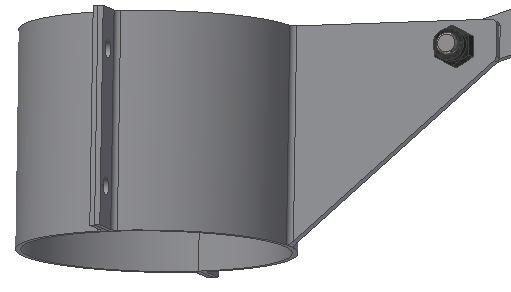
\includegraphics[width=0.4\textwidth]{Images/photos_PGA/collierSupport2.PNG}
    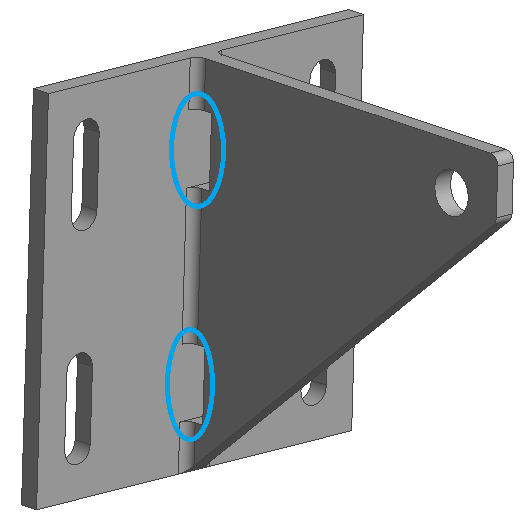
\includegraphics[width=0.3\textwidth]{Images/photos_PGA/supportmural2.PNG}
    \caption{Support de fixation tubulaire et mural}
    \label{fig:supfix}
\end{figure}

Un autre dispositif pour une fixation murale a aussi été pensé. Malheureusement dans cette configuration 
la rotation azimutale ne peut pas être réglée. Le seul degré de liberté est l’élévation. Les trous en 
bleus ont été pensé pour passer un éventuel collier de serrage pour un fixation spécial ou un montage 
provisoire.

\subsection{LoRaSnow Testbox}

Pour savoir si les simulations effectuées correspondaient avec la réalité, il a fallu tester le capteur 
en condition réel. Cependant les chutes de neiges sont difficilement prévisibles. Le boitier étant un 
concept mécanique, il fallait protéger les composants durant les essais. Un boitier pour la soirée de 
test a rapidement été fabriquer la veille pour protéger les composants électroniques de la neige. La 
fixation avec les clips a pu être expérimentée sous le boitier pour fixer le lidar. Ce type de fixation 
n’étant pas convainquant, un collier Colson fut rajouté pour augmenter la force de pincement des clips. 
Une autre fixation permettait de fixer le boitier sur un trépied.

\begin{figure}[H]
    \centering
    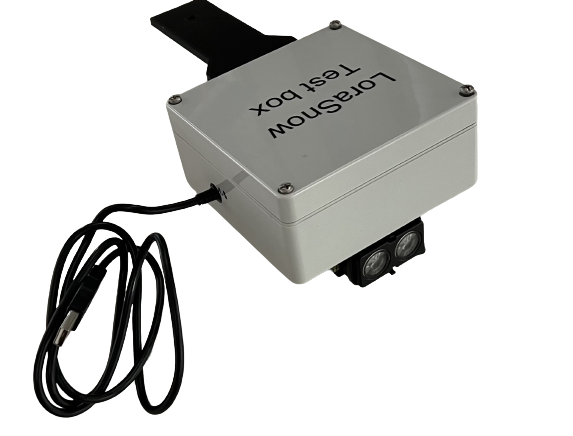
\includegraphics[width=0.45\textwidth]{Images/photos_PGA/TestBox-removebg-preview.png}
    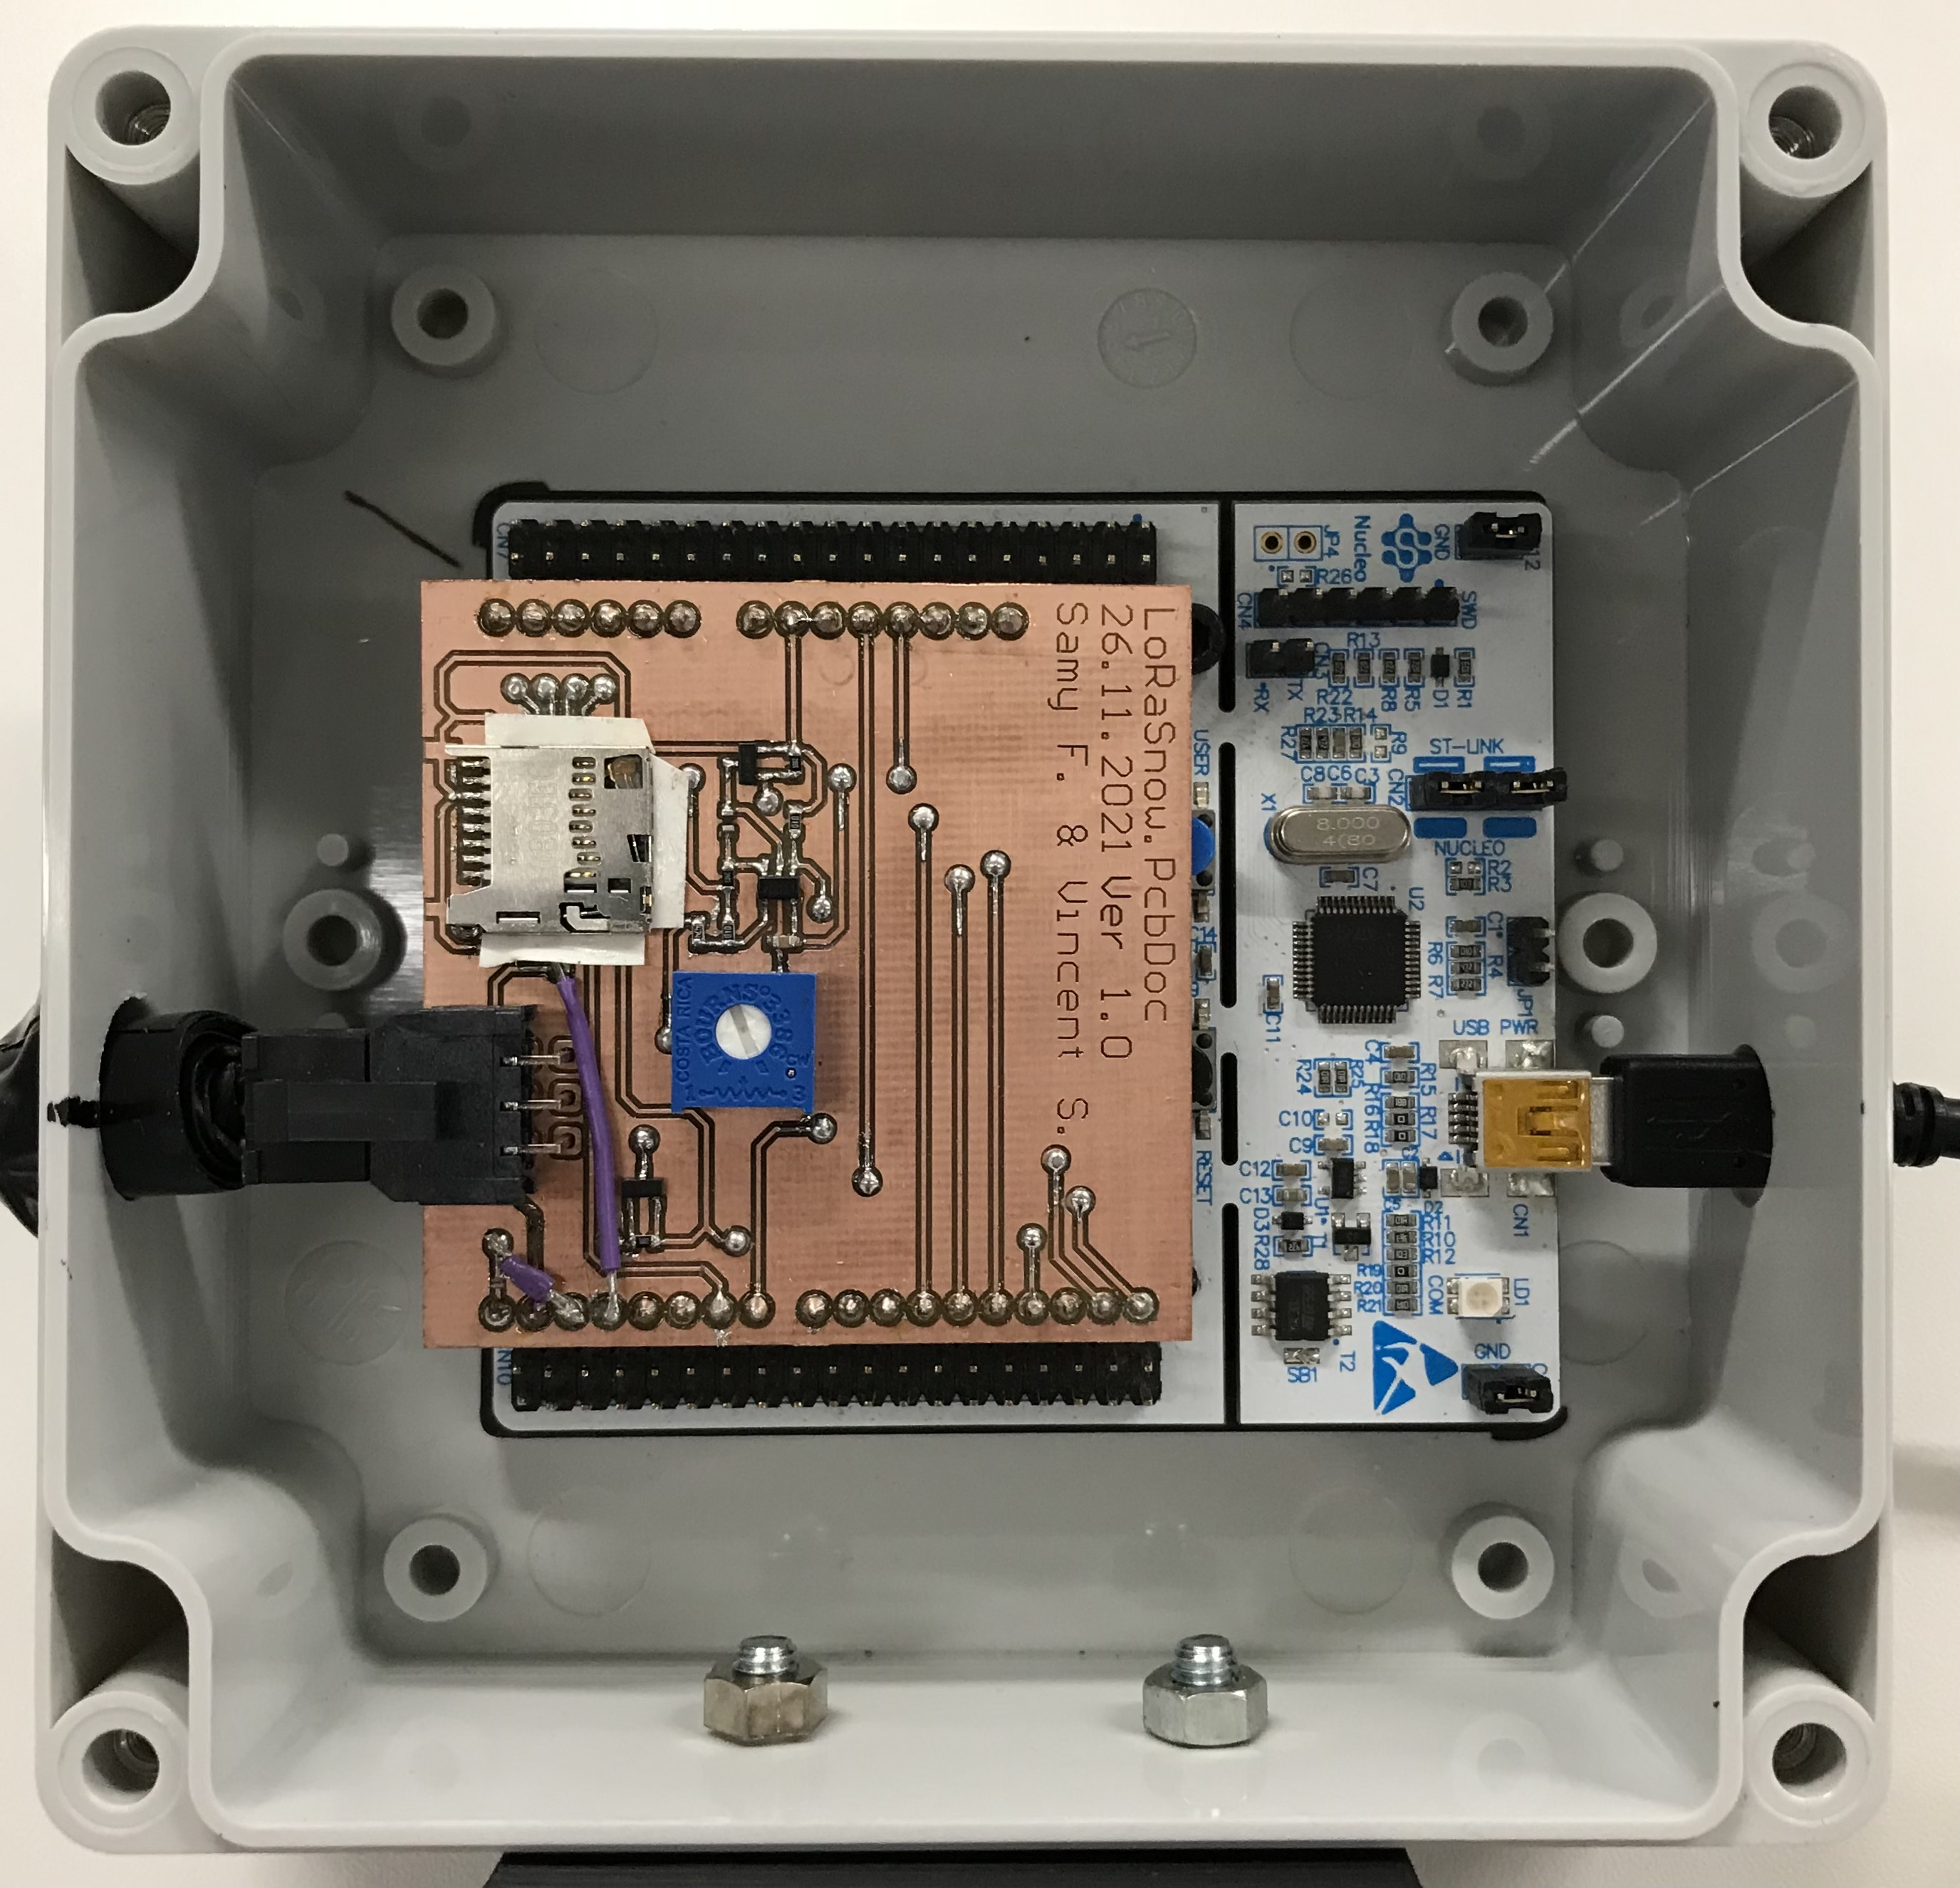
\includegraphics[width=0.35\textwidth]{Images/photos_PGA/testboxinside.jpg}
    \caption{LoRaSnow Testbox, intérieur et extérieur}
    \label{fig:testbox}
\end{figure}

